\documentclass[a4paper, 12pt]{article}

% --- PACOTES ---
% --- Codificação e Fontes ---
\usepackage[utf8]{inputenc}
\usepackage[T1]{fontenc}
\usepackage{lmodern}
\usepackage[brazil]{babel}
\usepackage{microtype}

% --- Layout e Estrutura ---
\usepackage{geometry}
\usepackage{graphicx}
\usepackage{float}

% --- Tabelas ---
\usepackage{array}
\usepackage{longtable}
\usepackage{booktabs}
\usepackage{ragged2e}

% --- Citações e Referências ---
\usepackage{natbib}

% --- Listas ---
\usepackage{enumitem}
\newlist{compactitem}{itemize}{1}
\setlist[compactitem]{label=\textbullet, topsep=0pt, partopsep=0pt, itemsep=0pt, parsep=0pt, leftmargin=*}

% --- Links ---
\usepackage[hidelinks]{hyperref}

\geometry{
    a4paper,
    left=2.5cm,
    right=2.5cm,
    top=2.5cm,
    bottom=2.5cm,
}

\graphicspath{{UGR16/figures/}}

\begin{document}

% --- PÁGINA DE ROSTO ---
\begin{titlepage}
    \centering
    
\includegraphics[width=0.4\textwidth]{upe.png}\par
    \vspace{1.5cm}

    {\large UNIVERSIDADE DE PERNAMBUCO - UPE}\par
    \vspace{0.2cm}
    {\large ESCOLA POLITÉCNICA DE PERNAMBUCO - POLI}

    \vfill

    {\Large \textbf{RELATÓRIO DE ANÁLISE EXPLORATÓRIA}}\par

    \vspace{1cm}

    {\huge \bfseries UGR'16 DATASET }\par

    \vfill

    \begin{flushleft}
    \large
        \textbf{Alunos:} Gabriel Souza Borges \\
        \textbf{Orientador:} Prof. Dr. Bruno José Torres Fernandes \\
    \end{flushleft}

    \vfill

    \large
    Recife-PE \\
    \today
\end{titlepage}

\tableofcontents
\listoffigures
\listoftables

\newpage

\section{Introdução}
O conjunto UGR'16 consiste em fluxos NetFlow coletados por um provedor de serviços de internet (ISP) espanhol ao longo de 2016, contendo tráfego legítimo e eventos maliciosos identificados por listas negras, detecções de botnet, varreduras SSH e outros sensores. Esta análise exploratória replica a metodologia aplicada ao CTU-13, amostrando exatamente 2{,}8 milhões de fluxos para permitir comparações equilibradas dos comportamentos de beaconing C2 no projeto \textit{Anomaly Detection in C2 Beaconing Traffic Using Privacy-Preserving Federated Learning}.

\section{Metodologia}
Amostramos exatamente 2{,}8 milhões de fluxos por meio de \textit{reservoir sampling} com semente fixa (42) no DuckDB, igualando o volume trabalhado com CTU-13 e garantindo reprodutibilidade. O resultado foi persistido em formato Parquet compactado com ZSTD. As etapas principais executadas no notebook \texttt{notebooks/eda\_ugr16.ipynb} foram:
\begin{compactitem}
    \item Carregamento eficiente do arquivo Parquet utilizando a biblioteca \texttt{fastparquet}.
    \item Renomear colunas automaticamente detectadas (\texttt{column00}--\texttt{column12}) para rótulos semânticos padronizados (\texttt{timestamp}, \texttt{src\_ip}, \texttt{dst\_ip}, \texttt{src\_port}, \texttt{dst\_port}, \texttt{protocol}, \texttt{flags}, \texttt{tos}, \texttt{packets\_fwd}, \texttt{packets\_bwd}, \texttt{bytes\_total}, \texttt{label}).
    \item Conversão de tipos para \texttt{datetime}, numéricos (\texttt{Int64}, \texttt{float}) e categóricos, otimizando memória e agregações.
    \item Derivação do indicador binário \texttt{is\_malicious} por correspondência de palavras-chave (\textit{botnet}, \textit{attack}, \textit{anomaly}, \textit{malicious}, \textit{ddos}, \textit{worm}, \textit{spam}, \textit{blacklist}), permitindo análises de contraste com tráfego benigno.
    \item Geração automatizada de figuras de alta resolução (300 DPI) em \texttt{docs/figures} e tabelas LaTeX em \texttt{docs/tables} para integração direta neste relatório.
\end{compactitem}

\section{Perfil do Tráfego}
A Figura~\ref{fig:ugr16_label_distribution} revela forte predominância de tráfego de fundo (\textit{background}), responsável por 96{,}7\% dos fluxos (2{,}7 milhões). O segundo rótulo mais frequente, \textit{anomaly-sshscan}, representa varreduras SSH detectadas como anomalia (83{,}062 fluxos, 3{,}0\%), seguido por eventos em lista negra (\textit{blacklist}, 9{,}946 fluxos, 0{,}4\%). Esse desbalanceamento extremo entre classes é característico de tráfego ISP real e exige estratégias específicas de aprendizado (reamostragem, perdas ponderadas) em modelos de detecção.

A Tabela~\ref{tab:ugr16_label_summary} detalha estatísticas de duração média, pacotes e bytes para os vinte rótulos mais frequentes. Observa-se que eventos de \textit{anomaly-sshscan} apresentam maior número médio de pacotes (18{,}4 vs. 9{,}6 no tráfego de fundo), enquanto fluxos em \textit{blacklist} exibem maior volume médio de bytes (21{,}034 vs. 15{,}360), sugerindo padrões volumétricos distintos úteis para caracterização.

\begin{figure}[H]
    \centering
    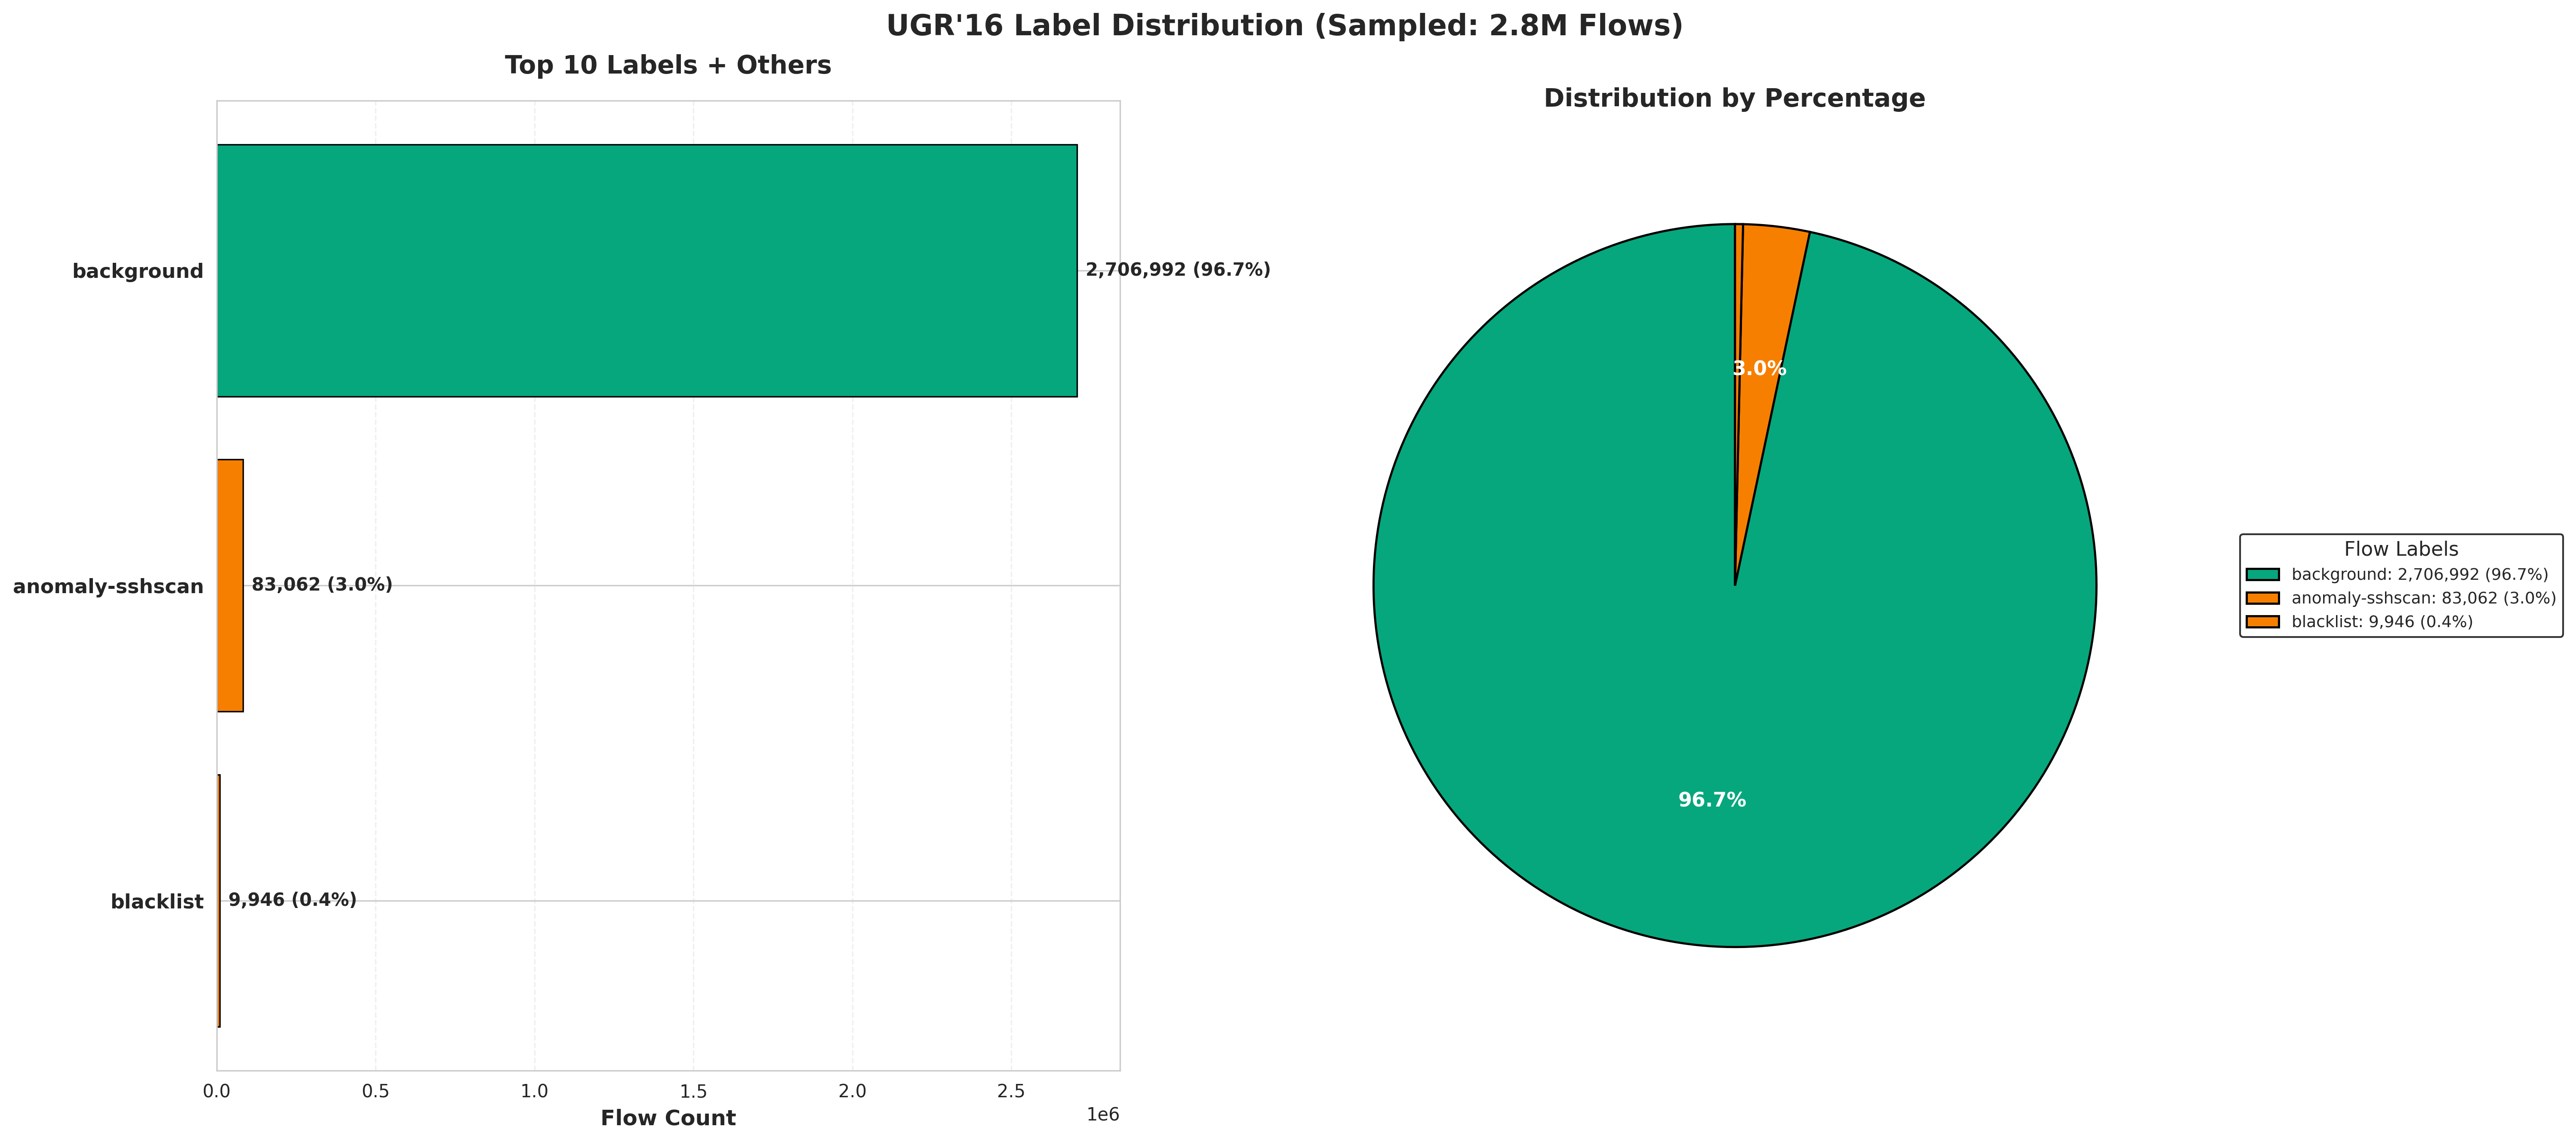
\includegraphics[width=0.98\textwidth]{ugr16_label_distribution.png}
    \caption{Distribuição dos rótulos no subconjunto amostrado do UGR'16. O painel esquerdo mostra contagens absolutas e percentuais; o painel direito apresenta a proporção visual. O tráfego de fundo domina com 96{,}7\% dos fluxos, enquanto anomalias SSH e eventos em lista negra representam a maior parte do tráfego malicioso detectado.}
    \label{fig:ugr16_label_distribution}
\end{figure}

\begin{longtable}{lrrrrr}
\caption{Top 20 Labels by Flow Count (UGR'16 Sample)} \label{tab:ugr16_label_summary} \\
\toprule
Label & Flows & Flow\_Percentage & Avg\_Duration\_s & Avg\_Total\_Packets & Avg\_Total\_Bytes \\
\midrule
\endfirsthead
\caption[]{Top 20 Labels by Flow Count (UGR'16 Sample)} \\
\toprule
Label & Flows & Flow\_Percentage & Avg\_Duration\_s & Avg\_Total\_Packets & Avg\_Total\_Bytes \\
\midrule
\endhead
\midrule
\multicolumn{6}{r}{Continued on next page} \\
\midrule
\endfoot
\bottomrule
\endlastfoot
background & 2706992 & 96.68 & 4.71 & 9.55 & 15,360.33 \\
anomaly-sshscan & 83062 & 2.97 & 3.24 & 18.37 & 1,278.46 \\
blacklist & 9946 & 0.36 & 2.91 & 13.02 & 21,034.05 \\
\end{longtable}


A Figura~\ref{fig:ugr16_protocol_port_profiles} mostra as principais distribuições de protocolos e portas de destino. O tráfego é dominado por TCP, seguido por UDP e ICMP, refletindo a composição típica de um ISP. As portas de destino mais frequentes incluem portas efêmeras (alta numeração) e serviços padrão como HTTP (80), HTTPS (443), DNS (53) e SSH (22). Essa heterogeneidade de serviços reforça a necessidade de normalização cuidadosa em experimentos federados. As Tabelas~\ref{tab:ugr16_protocol_summary} e \ref{tab:ugr16_top_ports} complementam com contagens absolutas e facilitam análises quantitativas.

\begin{figure}[H]
    \centering
    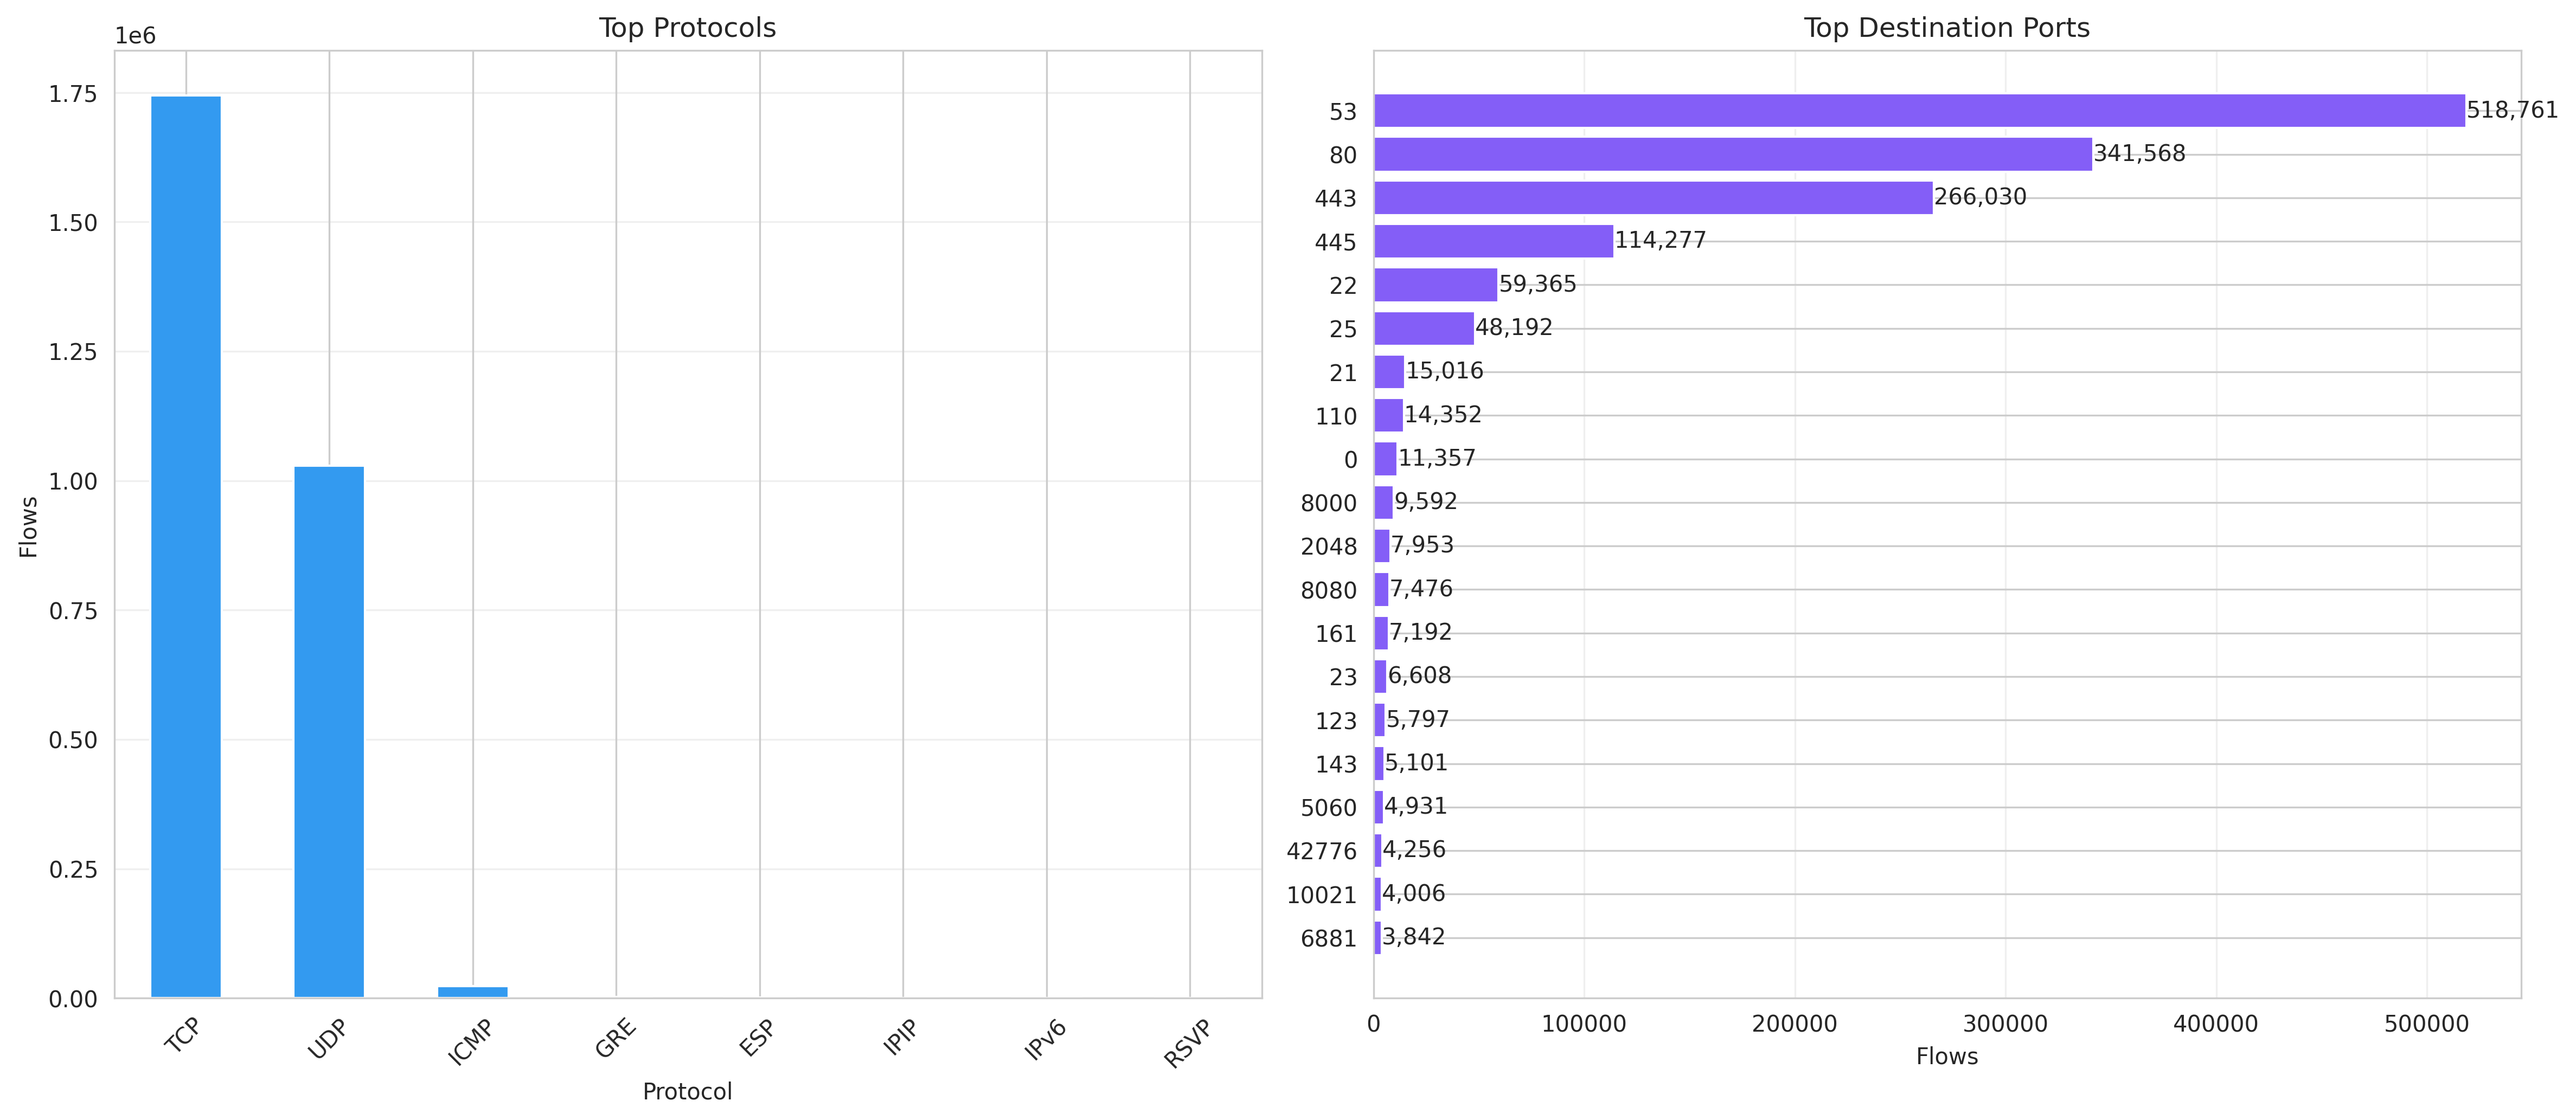
\includegraphics[width=0.98\textwidth]{ugr16_protocol_port_profiles.png}
    \caption{Distribuição de protocolos (painel esquerdo) e das 20 portas de destino mais frequentes (painel direito) no UGR'16. A predominância de TCP e a diversidade de portas evidenciam a heterogeneidade do tráfego ISP.}
    \label{fig:ugr16_protocol_port_profiles}
\end{figure}

\begin{table}
\caption{Protocol Frequency Summary (UGR'16 Sample)}
\label{tab:ugr16_protocol_summary}
\begin{tabular}{lr}
\toprule
protocol & Flows \\
\midrule
TCP & 1744403 \\
UDP & 1028764 \\
ICMP & 23284 \\
GRE & 2029 \\
ESP & 1151 \\
IPIP & 252 \\
IPv6 & 116 \\
RSVP & 1 \\
\bottomrule
\end{tabular}
\end{table}

\begin{table}
\caption{Top 20 Destination Ports (UGR'16 Sample)}
\label{tab:ugr16_top_ports}
\begin{tabular}{rr}
\toprule
Flows & count \\
\midrule
53 & 518761 \\
80 & 341568 \\
443 & 266030 \\
445 & 114277 \\
22 & 59365 \\
25 & 48192 \\
21 & 15016 \\
110 & 14352 \\
0 & 11357 \\
8000 & 9592 \\
2048 & 7953 \\
8080 & 7476 \\
161 & 7192 \\
23 & 6608 \\
123 & 5797 \\
143 & 5101 \\
5060 & 4931 \\
42776 & 4256 \\
10021 & 4006 \\
6881 & 3842 \\
\bottomrule
\end{tabular}
\end{table}


\section{Comparação Tráfego Malicioso vs. Benigno}
Aplicando o indicador \texttt{is\_malicious} derivado por palavras-chave, identificamos 93{,}008 fluxos maliciosos (3{,}3\% do total) contra 2{,}7 milhões de fluxos benignos. A Figura~\ref{fig:ugr16_attack_vs_background} compara duração, pacotes enviados (\textit{forward}), pacotes recebidos (\textit{backward}) e bytes totais entre os dois grupos, aplicando corte no 99º percentil para melhor visualização.

Fluxos maliciosos apresentam duração média menor (3{,}2s vs. 4{,}7s), maior número de pacotes enviados (17{,}8 vs. 9{,}6), porém menor volume total de bytes (3{,}391 vs. 15{,}360), conforme detalhado na Tabela~\ref{tab:ugr16_attack_background}. Esse perfil sugere comunicações curtas e intensivas (características de varreduras, tentativas de login automatizadas e beaconing C2 de baixo volume), contrastando com transferências de dados legítimas mais volumosas. Tais diferenças são promissoras para modelos de detecção baseados em estatísticas de fluxo.

\begin{figure}[H]
    \centering
    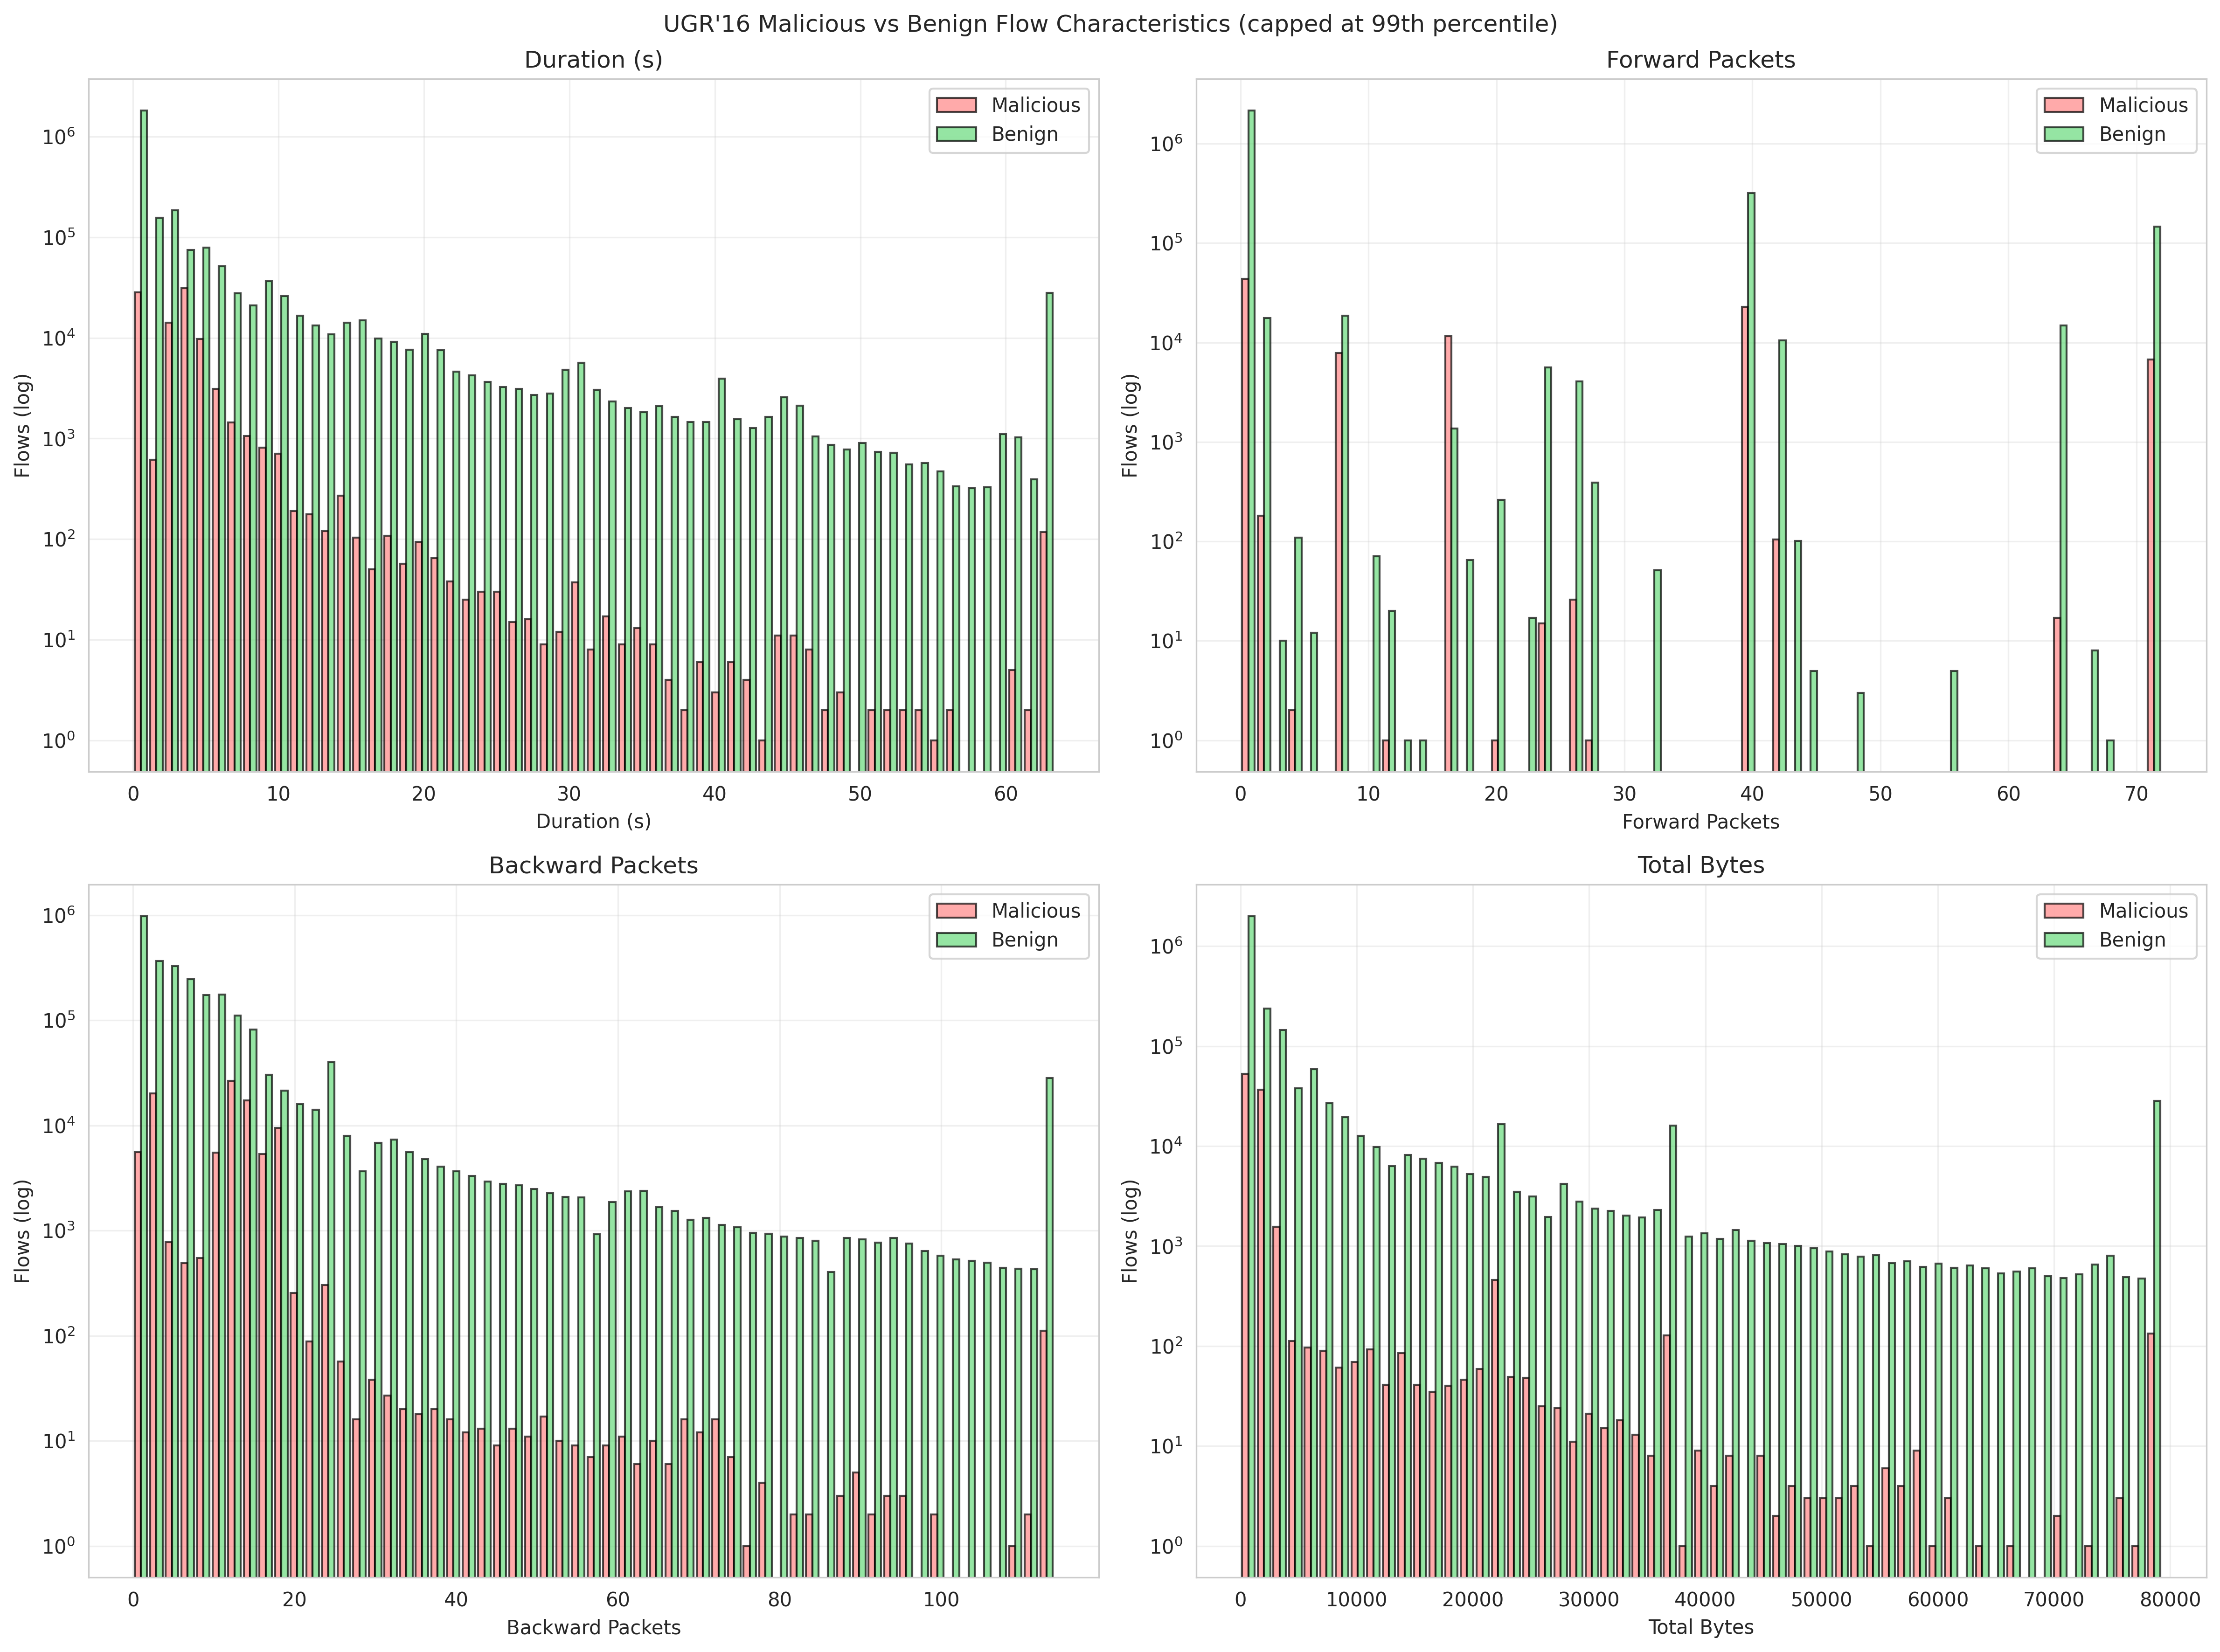
\includegraphics[width=0.98\textwidth]{ugr16_attack_vs_background.png}
    \caption{Características comparativas de fluxos maliciosos e benignos no UGR'16. Os histogramas mostram distribuições (escala logarítmica) limitadas ao 99º percentil para duração, pacotes enviados/recebidos e bytes totais. O painel inferior direito compara distribuição de protocolos entre as duas classes.}
    \label{fig:ugr16_attack_vs_background}
\end{figure}

\begin{table}
\caption{Malicious vs Benign Flow Statistics (UGR'16 Sample)}
\label{tab:ugr16_attack_background}
\begin{tabular}{lrrrrr}
\toprule
 & flows & avg\_duration & avg\_packets\_fwd & avg\_packets\_bwd & avg\_bytes \\
is\_malicious &  &  &  &  &  \\
\midrule
Benign & 2706992 & 4.71 & 9.55 & 22.21 & 15,360.33 \\
Malicious & 93008 & 3.20 & 17.80 & 11.96 & 3,391.07 \\
\bottomrule
\end{tabular}
\end{table}


\section{Padrões Temporais}
A série horária da Figura~\ref{fig:ugr16_hourly_activity} revela variações significativas de volume ao longo do período capturado, com picos que superam 20{,}000 fluxos por hora e vales próximos a zero, indicando possível descontinuidade na coleta ou janelas de baixa atividade. A Tabela~\ref{tab:ugr16_temporal_stats} sumariza estatísticas descritivas (média, mediana, percentis 90 e 99) da série temporal.

Quando segmentado pelo indicador de malícia (Figura~\ref{fig:ugr16_hourly_activity_by_label}), observam-se picos concentrados nos fluxos maliciosos em janelas específicas, sugerindo campanhas de ataque ou varreduras coordenadas. Esse padrão temporal pode orientar a detecção de beaconing periódico e a identificação de janelas de atividade anômala em cenários federados, permitindo que clientes detectem surtos locais sem compartilhar dados crus.

\begin{figure}[H]
    \centering
    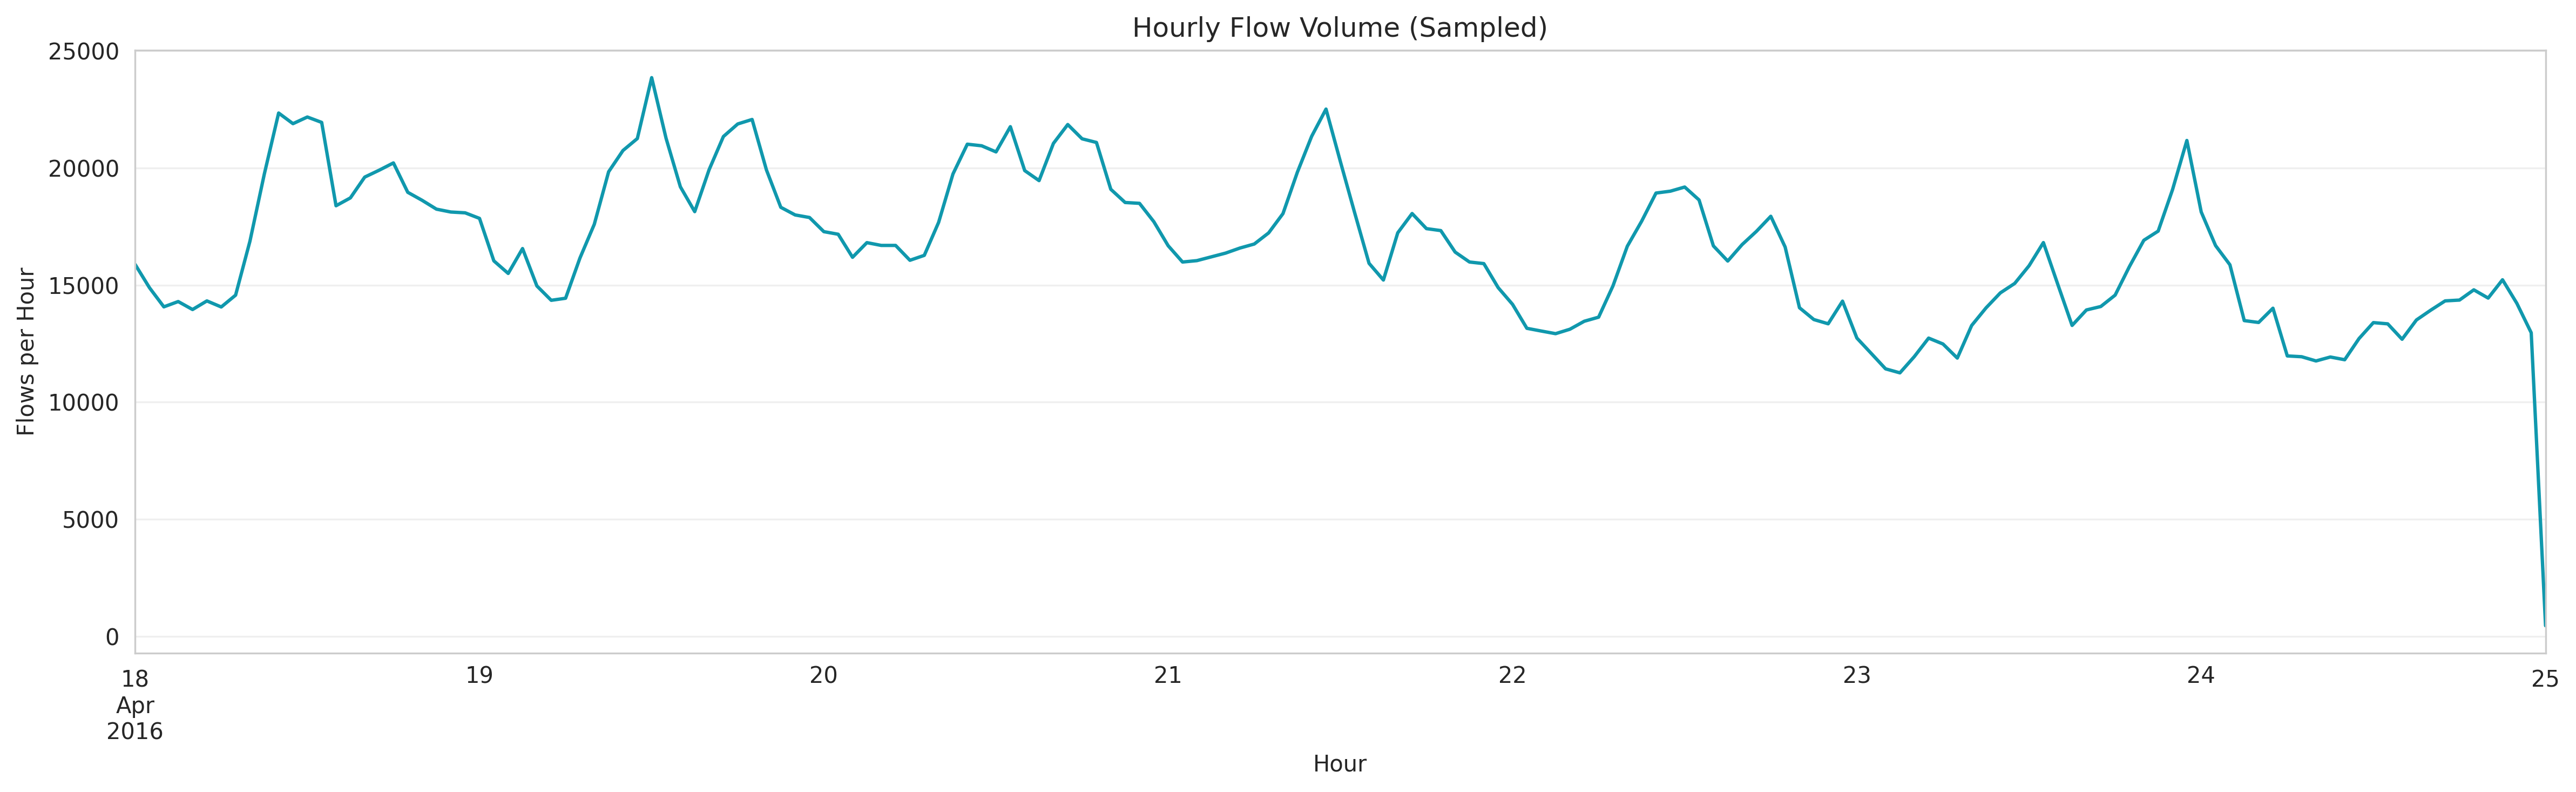
\includegraphics[width=0.98\textwidth]{ugr16_hourly_activity.png}
    \caption{Volume horário de fluxos no subconjunto do UGR'16. As variações acentuadas indicam padrões de atividade heterogêneos ao longo do período amostrado.}
    \label{fig:ugr16_hourly_activity}
\end{figure}

\begin{figure}[H]
    \centering
    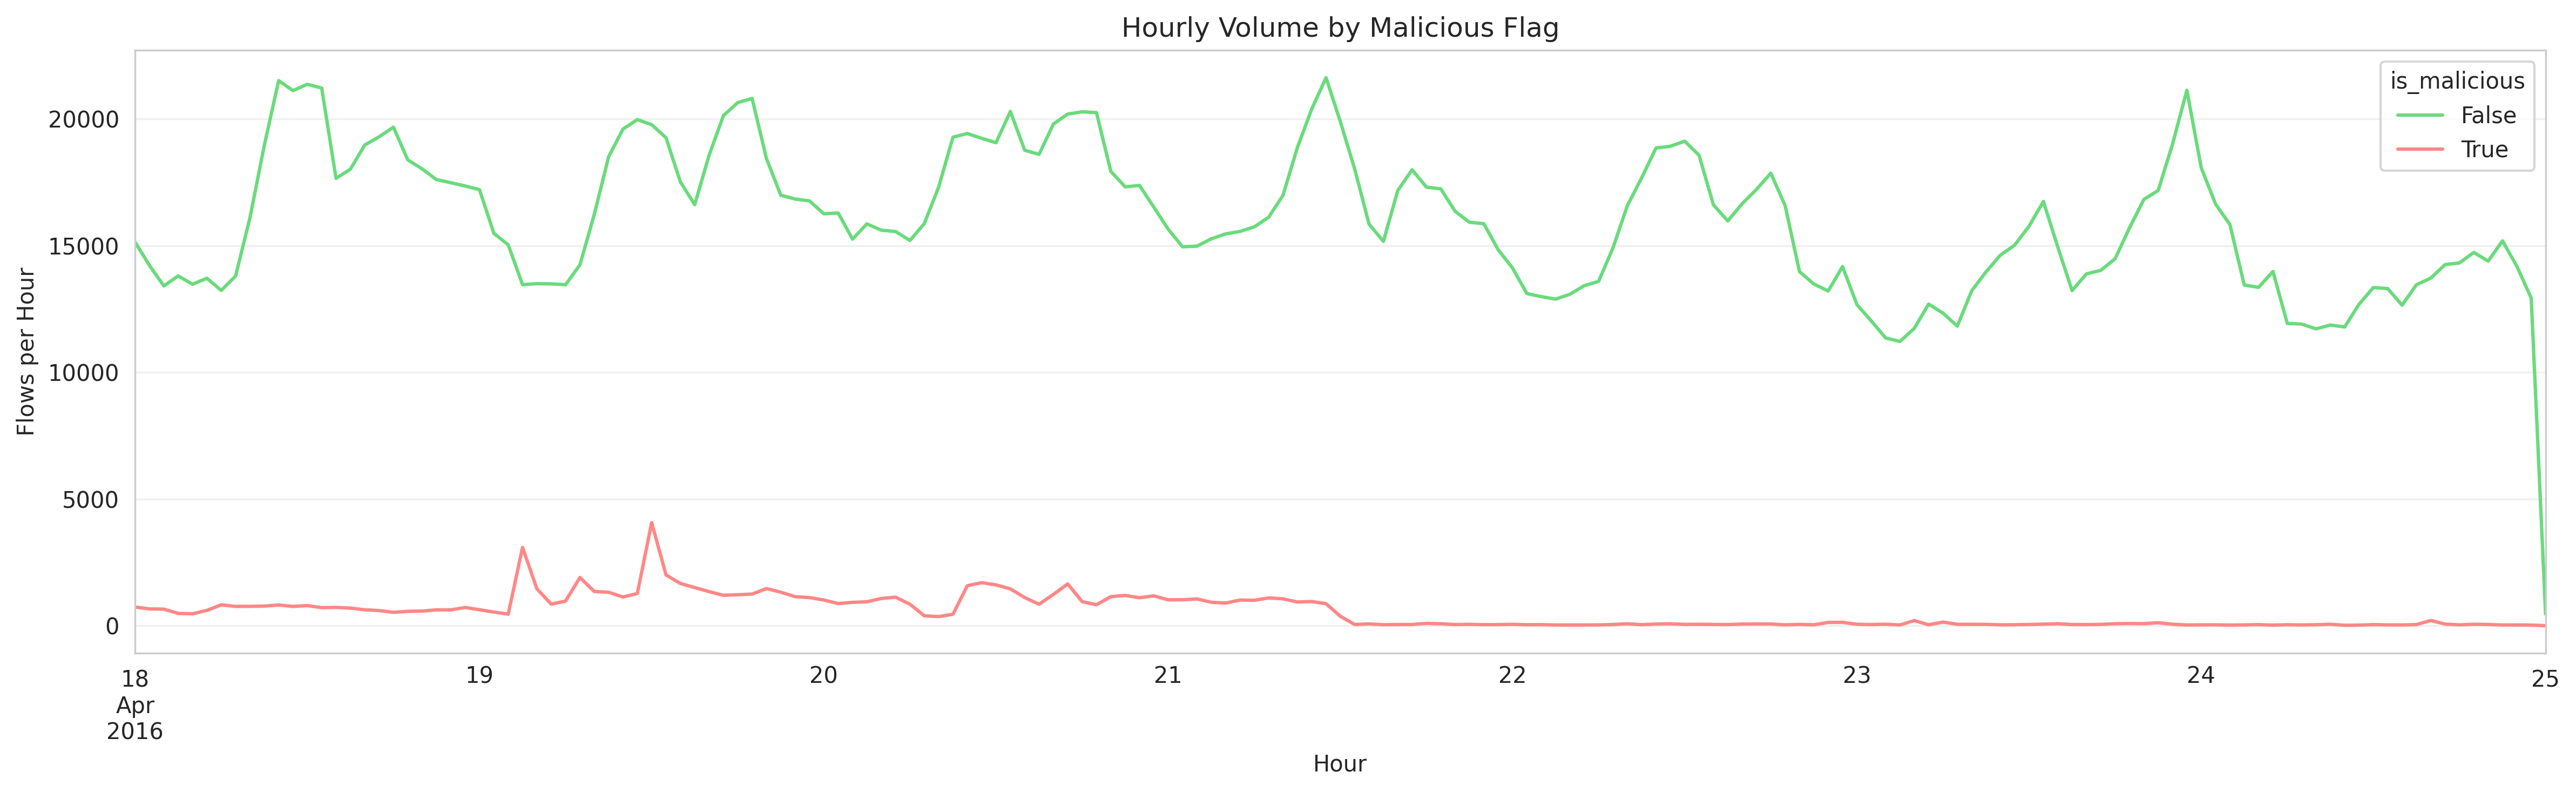
\includegraphics[width=0.98\textwidth]{ugr16_hourly_activity_by_label.png}
    \caption{Volume horário segmentado por indicador malicioso/benigno. Os picos de tráfego malicioso concentrados em janelas específicas sugerem campanhas de ataque ou varreduras automatizadas.}
    \label{fig:ugr16_hourly_activity_by_label}
\end{figure}

\begin{table}
\caption{Hourly Flow Volume Summary (UGR'16 Sample)}
\label{tab:ugr16_temporal_stats}
\begin{tabular}{lr}
\toprule
 & Flows per Hour \\
\midrule
count & 169.00 \\
mean & 16,568.05 \\
std & 3,172.03 \\
min & 460.00 \\
25% & 14,218.00 \\
50% & 16,622.00 \\
75% & 18,630.00 \\
max & 23,850.00 \\
\bottomrule
\end{tabular}
\end{table}


\section{Correlações entre Variáveis}
A matriz de correlação apresentada na Figura~\ref{fig:ugr16_numeric_correlation} mostra dependências positivas fortes entre \texttt{packets\_fwd} (pacotes enviados) e \texttt{bytes\_total} (correlação esperada, dado que mais pacotes implicam maior volume), bem como correlação moderada entre \texttt{packets\_fwd} e \texttt{packets\_bwd} (tráfego bidirecional). A variável \texttt{duration} exibe correlações mais fracas com as demais, sugerindo que fluxos longos não necessariamente transferem grandes volumes.

Essas observações reforçam a necessidade de incorporar métricas temporais derivadas (intervalos de beaconing, periodicidade, jitter, entropia de portas/protocolos) nas próximas fases do estudo, uma vez que atributos volumétricos brutos podem não capturar completamente padrões de comunicação C2 que operam em rajadas curtas e regulares.

\begin{figure}[H]
    \centering
    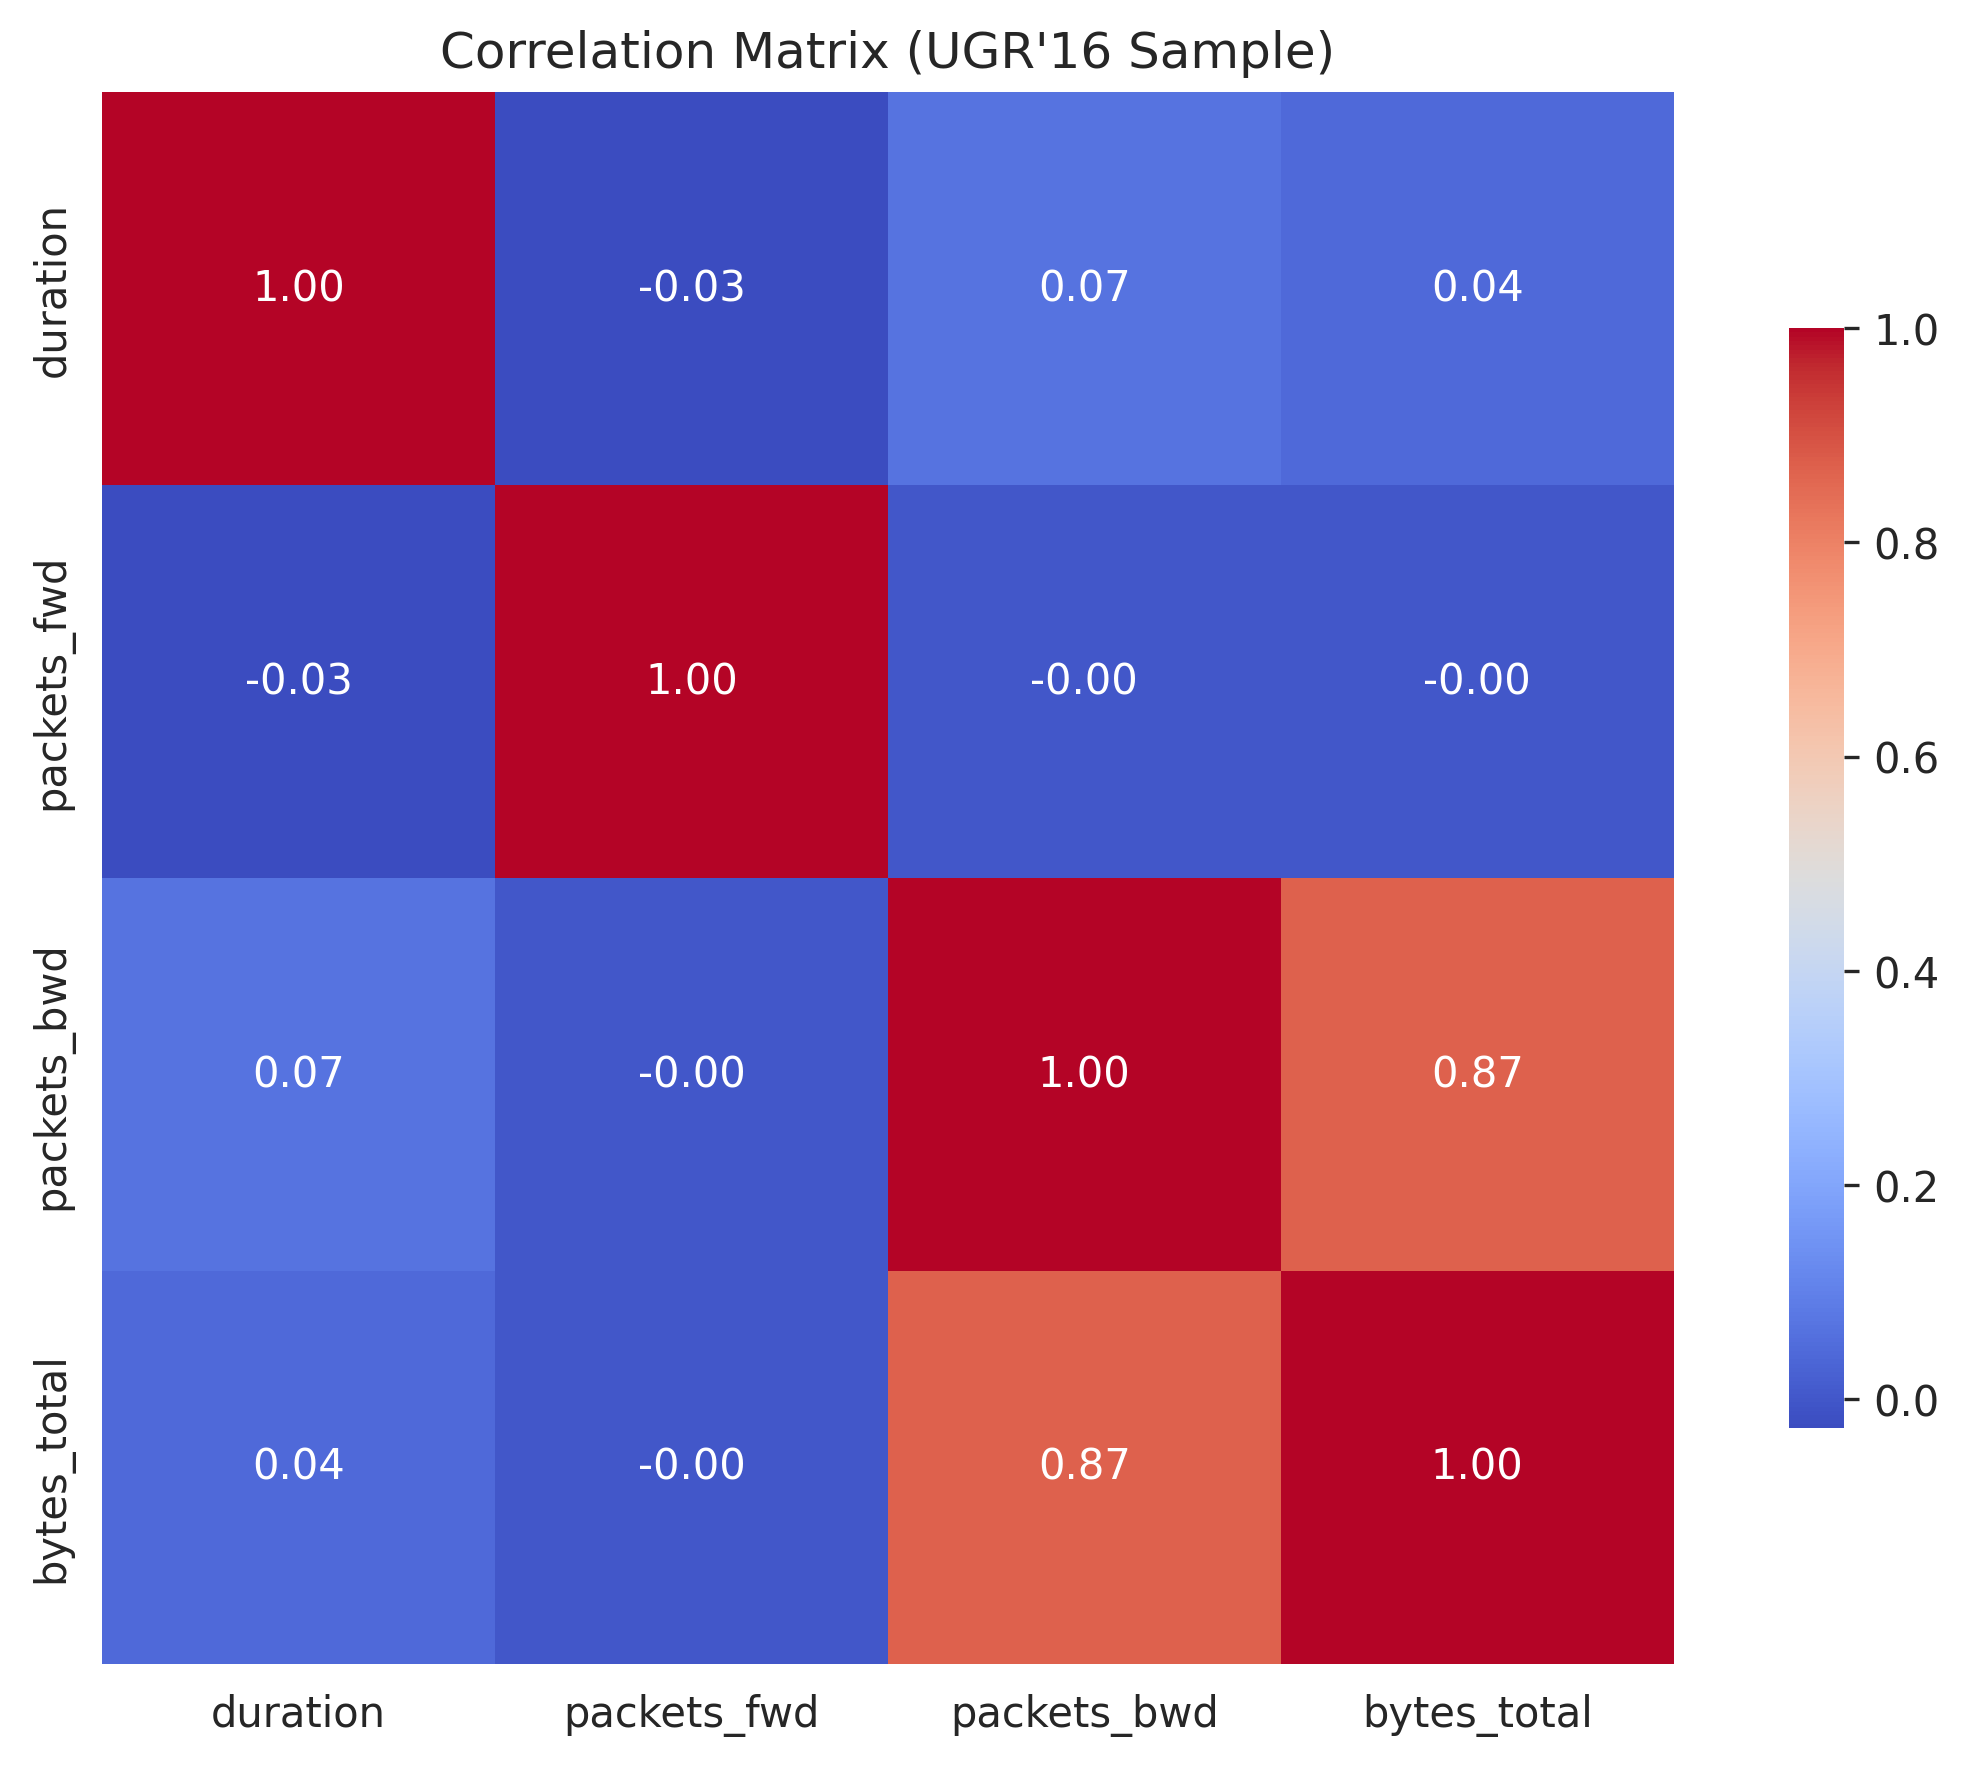
\includegraphics[width=0.80\textwidth]{ugr16_numeric_correlation.png}
    \caption{Matriz de correlação para atributos numéricos do UGR'16. Observam-se correlações positivas entre volume de pacotes e bytes, enquanto a duração apresenta dependências mais fracas.}
    \label{fig:ugr16_numeric_correlation}
\end{figure}

\section{Implicações para Aprendizado Federado}
Os resultados obtidos nesta análise exploratória orientam o desenho de experimentos federados em múltiplas dimensões:

\begin{compactitem}
    \item \textbf{Particionamento de clientes:} A diversidade de rótulos e protocolos sugere a construção de clientes federados baseados em perfis de tráfego (ISP corporativo, backbone, honeypots, redes acadêmicas), cada qual retendo seu subconjunto amostrado. Essa heterogeneidade é fundamental para avaliar a robustez de modelos treinados em cenários não-IID.
    
    \item \textbf{Desbalanceamento de classes:} Com 96{,}7\% de fluxos benignos, o dataset exige estratégias específicas: reamostragem (undersampling de background, oversampling de maliciosos), funções de perda ponderadas (Focal Loss, Class-Balanced Loss), ou técnicas de aprendizado com rótulos positivos raros (PU Learning, anomaly detection one-class).
    
    \item \textbf{Normalização e privacidade:} A variedade de protocolos e portas reforça a necessidade de esquemas de normalização consistentes entre clientes (z-score, min-max por cliente, ou agregações estatísticas seguras). Mecanismos de privacidade diferencial podem ser aplicados nos gradientes locais antes do envio ao servidor.
    
    \item \textbf{Refinamento do indicador malicioso:} O indicador binário \texttt{is\_malicious} pode ser refinado com listas adicionais (IPs de C2 conhecidos, assinaturas de malware), heurísticas específicas do domínio (entropia de payloads, padrões de User-Agent), e validação cruzada com feeds de threat intelligence.
\end{compactitem}

\section{Próximos Passos}
\begin{compactitem}
    \item \textbf{Engenharia de atributos temporais:} Derivar métricas de beaconing (intervalos entre fluxos consecutivos do mesmo par IP, periodicidade via FFT, jitter, coeficiente de variação) e entropia (distribuição de portas/protocolos por host).
    
    \item \textbf{Expansão da amostragem:} Incorporar diferentes semanas/meses do UGR'16 para avaliar sazonalidade, drift temporal e robustez do indicador malicioso em períodos distintos.
    
    \item \textbf{Validação e refinamento de labels:} Cruzar o indicador \texttt{is\_malicious} com feeds de threat intelligence externos (Abuse.ch, VirusTotal, AbuseIPDB) e ajustar a lista de palavras-chave para minimizar falsos positivos/negativos.
    
    \item \textbf{Experimentos federados cross-dataset:} Projetar configurações combinando CTU-13 (cenários de botnet controlados) e UGR'16 (tráfego ISP real), testando generalização cruzada, transferência de conhecimento e estratégias de preservação de privacidade (Differential Privacy, Secure Aggregation, Homomorphic Encryption).
    
    \item \textbf{Baseline de modelos:} Treinar classificadores clássicos (Random Forest, XGBoost, Isolation Forest) e redes neurais (MLP, LSTM para séries temporais) em configuração centralizada, estabelecendo métricas de referência (F1-score, AUC-ROC, precisão@k) antes de avaliar abordagens federadas.
\end{compactitem}

\section{Conclusão}
A análise exploratória do UGR'16 complementa os achados do CTU-13 ao oferecer um ambiente ISP realista com forte desbalanceamento de classes (96{,}7\% tráfego benigno vs. 3{,}3\% malicioso), diversidade de protocolos e serviços, e padrões temporais de ataque concentrados em janelas específicas. O subconjunto amostrado de 2{,}8 milhões de fluxos fornece base consistente e reprodutível para desenhar e avaliar detectores de beaconing C2 em cenários federados.

As diferenças observadas entre fluxos maliciosos e benignos---duração reduzida, maior taxa de pacotes enviados, menor volume total---são compatíveis com comunicações de comando-e-controle e varreduras automatizadas, validando a relevância do dataset para o problema de pesquisa. Os próximos passos envolvem engenharia de atributos temporais, particionamento não-IID de clientes federados, e integração de mecanismos de privacidade diferencial para garantir proteção de dados sensíveis durante o treinamento colaborativo.

\end{document}
